\documentclass[sigplan,authorversion]{acmart}

\usepackage{booktabs}
\usepackage{subcaption}

% Haskell code snippets and useful shortcuts
\usepackage{minted}
\setminted[haskell]{escapeinside=@@}
\newcommand{\hs}{\mintinline{haskell}}
\newcommand{\teq}{\smaller $\sim$}
\newcommand{\ghci}{$\lambda$>}
\newcommand{\defeq}{\stackrel{\text{def}}{=}}
\newcommand{\std}[1]{{\color[rgb]{0,0.3,0} #1}}
\newcommand{\blk}[1]{{\color[rgb]{0,0,0} #1}}

\makeatletter

\setcopyright{acmlicensed}
\acmDOI{10.1145/3122955.3122956}
\acmISBN{978-1-4503-5182-9/17/09}
\acmConference[Haskell'17]{10th ACM SIGPLAN International Haskell Symposium}{September 7-8, 2017}{Oxford, UK}
\acmYear{2017}
\copyrightyear{2017}
\acmPrice{15.00}

\bibliographystyle{ACM-Reference-Format}
\citestyle{acmauthoryear}

\begin{document}
\settopmatter{printacmref=false}
\title{Algebraic Graphs with Class\vspace{-1.5mm}}
\subtitle{Functional Pearl}

\author{Andrey Mokhov}
\affiliation{
  \institution{Newcastle University, United Kingdom\vspace{-1mm}}
}

\begin{abstract}
% \vspace{-1mm}
The paper presents a minimalistic and elegant approach to working
with graphs in Haskell. It is built on a rigorous
mathematical foundation --- an algebra of graphs --- that allows us to apply
equational reasoning for proving the correctness of graph transformation
algorithms. Algebraic graphs let us avoid partial functions typically
caused by `malformed graphs' that contain an edge referring to
a non-existent vertex. This helps to liberate APIs of existing graph libraries
from partial functions.

The algebra of graphs can represent directed, undirected, reflexive
and transitive graphs, as well as hypergraphs, by appropriately choosing
the set of underlying axioms. The flexibility of the approach is
demonstrated by developing a library for constructing
and transforming polymorphic graphs.
\end{abstract}

%% 2012 ACM Computing Classification System (CSS) concepts
%% Generate at 'http://dl.acm.org/ccs/ccs.cfm'.
\begin{CCSXML}
<ccs2012>
<concept>
<concept_id>10002950.10003624.10003633</concept_id>
<concept_desc>Mathematics of computing~Graph theory</concept_desc>
<concept_significance>500</concept_significance>
</concept>
\end{CCSXML}

\ccsdesc[500]{Mathematics of computing~Graph theory}
%\keywords{\vspace{-2mm}Haskell, algebra, graph theory}
\keywords{Haskell, algebra, graph theory}

\maketitle

%!TEX root = alga.tex
\section{Introduction}\label{sec-intro}

Graphs are ubiquitous in computing, yet working with graphs often requires
painfully low-level fiddling with sets of vertices and edges. Building
high-level abstractions is difficult, because the commonly used
foundation -- the pair $(V, E)$ of vertex set $V$ and edge set $E$ -- is a source
of partial functions. If $E \nsubseteq V \times V$, the pair is inconsistent and
does not correspond to a graph. This inherent partiality often leaks through
abstractions in state-of-the-art Haskell\footnote{In this paper
we exclusively use Haskell, but the presented approach can be adapted to other
programming languages.} graph libraries.

For example, the \textsf{containers} library represents graphs by
\emph{adjacency arrays}~\cite{1995_king_graphs}. To construct a graph
one specifies the pair $(V,E)$, e.g.
\hs{buildG (1,3) [(1,2),(2,3)]} constructs the graph with $V=\{1,2,3\}$ and
$E=\{(1,2), (2,3)\}$. Note that \hs{buildG} is partial:
\hs{buildG (1,2) [(3,1)]} is well-typed but fails with the
\textsf{`index out of range'} error. Another popular library \textsf{fgl}
uses the \emph{inductive graph representation} by~\citet{2001_erwig_inductive},
but its graph construction API is also based on sets of vertices and edges and
has partial functions, e.g. \hs{insEdge} can fail with
the \textsf{`edge from non-existent vertex'} error. Both \textsf{containers}
and \textsf{fgl} are treasure troves of graph algorithms, but it is easy to make an
error when using them. One can wrap these libraries in a safe interface, but the
question is: What is the right interface for constructing graphs? Is there a better
foundation than the pair $(V, E)$?

We present \emph{algebraic graphs} --- a new interface
for graph construction and transformation. We abstract away from graph representation
details and characterise graphs and two operations on them by a set of axioms,
much like numbers with addition and multiplication are algebraically characterised
by \emph{rings}~\cite{1999_maclane_algebra}. The presented approach is inspired by the
\emph{algebra of parameterised graphs}, a mathematical formalism used in digital
circuit design~\cite{2014_algebra_mokhov}, which we distil and adapt to the context
of functional programming.

The two binary operations on algebraic graphs, called \emph{overlay} and \emph{connect},
have two important properties: i) they are closed on the set of graphs, i.e. are total
functions, and ii) they can be used to construct any graph starting from the \emph{empty} and
single-\emph{vertex} graphs. This leads us to the safe and minimalistic core of four graph
construction primitives, as captured by the following data type:

\begin{minted}{haskell}
data Graph a = Empty
             | Vertex a
             | Overlay (Graph a) (Graph a)
             | Connect (Graph a) (Graph a)
\end{minted}

\noindent
To make the core more reusable we also define the following type class\footnote{The
name collision is not a problem in practice, because the data type and type class
are not used together and can be defined in separate modules.}, whose
instances must obey the axioms of the algebra:

\begin{minted}{haskell}
class Graph g where
    type Vertex g
    empty   :: g
    vertex  :: Vertex g -> g
    overlay :: g -> g -> g
    connect :: g -> g -> g
\end{minted}

\noindent
The main idea of the paper is that this simple core is as a solid foundation for
working with graphs. The type class has classic inhabitants, such as the pair $(V,E)$,
data types from \textsf{containers} and \textsf{fgl}, as well as new, unknown forms
of life. Our contributions are:
\begin{itemize}
  \item Compared to existing libraries, algebraic graphs have a smaller
  core (just four graph construction primitives), are more compositional
  (hence greater code reuse), and have no partial functions (hence fewer
  opportunities for usage errors). We present the core and justify these claims
  in \S\ref{sec-core}.

  \item The core has a simple mathematical structure fully characterised
  by a set of axioms~(\S\ref{sec-algebra}). This makes the
  proposed interface easier for testing and formal verification. We show that
  the core is \emph{complete}, i.e. any graph can be constructed, and \emph{sound},
  i.e. malformed graphs cannot be constructed.

  \item Under the basic set of axioms, algebraic graphs correspond to directed
  graphs with no edge labels. As we show in~\S\ref{sec-a-la-carte}, by extending
  the algebra
  with additional axioms, it is possible to also represent undirected, reflexive
  and transitive graphs, their combinations, as well as hypergraphs.
%   Importantly, the core
%   graph construction primitives remain unchanged, which allows to define highly
%   reusable polymorphic functions on graphs.

  \item We develop a library\footnote{The library is on Hackage:
  \url{http://hackage.haskell.org/package/algebraic-graphs}.} for polymorphic graph
  construction and transformation on top of the algebraic core and
  demonstrate its flexibility in \S\ref{sec-transformations}.
  % Although the development of efficient algorithms for algebraic
  % graphs is outside the scope of this paper, we show that the library can cope
  % with graphs comprising billions of edges in the matter of
  % seconds, which is sufficiently fast for many applications.
\end{itemize}

Graphs and functional programming have a long history. We review related
work in \S\ref{sec-related}. Limitations of this work and future
research directions are discussed in \S\ref{sec-discussion}.

%!TEX root = alga.tex
\section{The core}\label{sec-core}

In this section we define the \emph{core} of algebraic graphs -- a minimal set
of graph construction primitives that are compositional and total. The core is
built on the \emph{algebra of parameterised graphs}, a mathematical formalism
used in hardware design~\cite{2014_algebra_mokhov},
which we distil and adapt to the context of graph representation in functional
programming languages.

Let $G$ be a set of unlabelled directed graphs whose vertices come from a fixed
universe $\mathbb{V}$. As an example, we can think of graphs whose vertices are
positive integers. A graph $g \in G$ can be represented by a pair $(V, E)$ where
$V\subseteq \mathbb{V}$ is the set of its vertices and $E \subseteq V \times V$ is
the set of its edges.
If $E \nsubseteq V \times V$, then the pair $(V, E)$ is inconsistent and does not
correspond to a graph, which often leads to partial functions, as discussed
in \S\ref{sec-motivation}.

When one needs to guarantee the internal consistency of a data structure, such
as the pair $(V, E)$, the standard solution is to define an abstract interface
that encapsulates the data structure and provides a set of safe construction
primitives. This is exactly the approach we take in this paper.

\subsection{Constructing graphs}\label{sub-constructing}

The simplest possible graph is the \emph{empty} graph. We will denote it by
$\varepsilon$, therefore $\varepsilon = (\varnothing, \varnothing)$ and
$\varepsilon \in G$. A graph with a \emph{single vertex} $v \in \mathbb{V}$
will be denoted simply by $v$. For example, $1 \in G$ is the graph
$({1}, \varnothing)$.

To construct larger graphs from the above primitives we define binary
operations \emph{overlay} and \emph{connect}, denoted by $+$ and $\rightarrow$,
respectively. The overlay operation $+$ is defined as
\[
(V_1, E_1) + (V_2, E_2)~~\defeq~~(V_1 \cup V_2, E_1 \cup E_2).
\]
That is, the overlay of two graphs comprises the union of their vertices and edges.

The connect $\rightarrow$ operation is defined in a similar manner:
\[
(V_1, E_1) \rightarrow (V_2, E_2)~~\defeq~~(V_1 \cup V_2, E_1 \cup E_2 \cup V_1 \times V_2).
\]
The difference is that when we connect two graphs, an edge is added from each
vertex of the left-hand argument to each vertex of the right-hand
argument\footnote{Our definitions of overlay and connect coincide
with those of graph \emph{union} and \emph{join}, respectively,
e.g see~\citet{1969_graph_theory_harary},
however the arguments of union and join are typically assumed to have disjoint
sets of vertices. We make no such assumptions, hence our definitions are total:
any two graphs can be composed using overlay and connect.
}.
Note that the connect operation is the only source of edges when constructing
graphs. As we will see in \S\ref{sec-algebra}, the overlay and connect are very
similar to addition and multiplication, therefore connect has a higher
precedence, i.e. $1 + 2 \rightarrow 3$ is interpreted as $1 + (2 \rightarrow 3)$.

\noindent
Fig.~\ref{fig-construction} illustrates a few examples of constructing graphs
using the defined primitives:
\begin{itemize}
  \item $1 + 2$ is the graph with two isolated vertices 1 and 2.
  \item $1 \rightarrow 2$ is the graph with an edge between vertices 1
  and 2, i.e. the graph $a$ from Fig.~\ref{fig-example}.
  \item $1 \rightarrow (2 + 3)$ is the graph with three vertices $\{1, 2, 3\}$
  and two edges $(1, 2)$ and $(1, 3)$.
  \item $1 \rightarrow 1$ is the graph with vertex 1 and the \emph{self-loop}
  going from the vertex to itself.
  \item $1 \rightarrow 2 + 3 \rightarrow 1$ is the graph $b$ from
  Fig.~\ref{fig-example}.
\end{itemize}

\begin{figure}
\hspace{-5mm}
\begin{subfigure}[b]{0.2\linewidth}
\centerline{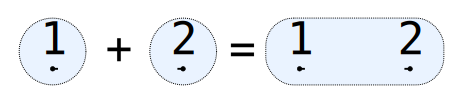
\includegraphics[scale=0.27]{fig/ex-a.pdf}}
\vspace{-2.4mm}
\caption{$1 + 2$}
\centerline{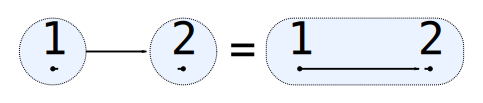
\includegraphics[scale=0.27]{fig/ex-b.pdf}}
\vspace{-2.4mm}
\caption{$1 \rightarrow 2$}
\end{subfigure}
\hspace{11mm}
\begin{subfigure}[b]{0.17\linewidth}
\centerline{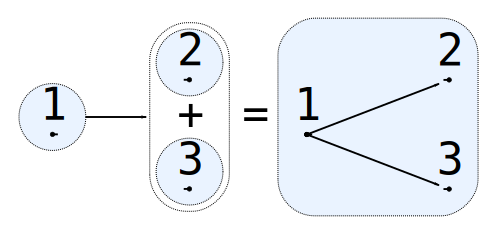
\includegraphics[scale=0.27]{fig/ex-c.pdf}}
\vspace{-1mm}
\caption{$1 \rightarrow (2 + 3)$}
\end{subfigure}
\hspace{12mm}
\begin{subfigure}[b]{0.15\linewidth}
\centerline{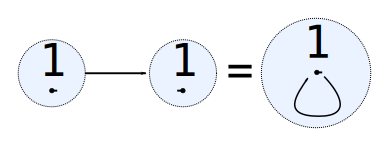
\includegraphics[scale=0.27]{fig/ex-d.pdf}}
\vspace{2.4mm}
\caption{$1 \rightarrow 1$}
\end{subfigure}
\hspace{12mm}
\begin{subfigure}[b]{0.2\linewidth}
\centerline{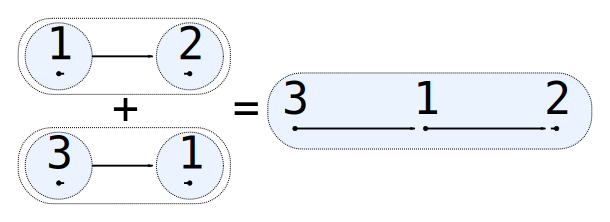
\includegraphics[scale=0.27]{fig/ex-e.pdf}}
\vspace{-1mm}
\caption{$1 \rightarrow 2 + 3 \rightarrow 1$}
\end{subfigure}
\vspace{-1mm}
\caption{Examples of graph construction\label{fig-construction}}
\vspace{-3mm}
\end{figure}

\vspace{-1mm}
\subsection{Type class}\label{sub-class}

We abstract the graph construction primitives defined in \S\ref{sub-constructing}
as the type class \hs{Graph}:

\begin{minted}{haskell}
class Graph g where
    type Vertex g
    empty   :: g
    vertex  :: Vertex g -> g
    overlay :: g -> g -> g
    connect :: g -> g -> g
\end{minted}

\noindent
Here the associated type\footnote{Associated
types~\cite{2005_associated_type_chakravarty} require the \textsf{TypeFamilies}
GHC extension.} \hs{Vertex@\,@g} corresponds to the universe of graph
vertices $\mathbb{V}$, \hs{empty} is the empty graph
$\varepsilon$, \hs{vertex} constructs a graph with a single vertex,
and \hs{overlay} and \hs{connect} compose given graphs according to
the definitions in~\S\ref{sub-constructing}. All methods of the type class
are total, i.e. are defined for all possible inputs, therefore,
the presented API allows \emph{fewer opportunities for usage errors}
and \emph{greater opportunities for reuse}.

Let's put the API to the test and construct some graphs! A single edge is
obtained by connecting two vertices:

\begin{minted}{haskell}
edge :: Graph g => Vertex g -> Vertex g -> g
edge x y = connect (vertex x) (vertex y)
\end{minted}

\noindent
The graphs in Fig.~\ref{fig-construction}(b,d) are \hs{edge@\,@1@\,@2} and
\hs{edge@\,@1@\,@1}, respectively.
A graph that contains a given list of isolated vertices can be constructed
as follows:

\begin{minted}{haskell}
vertices :: Graph g => [Vertex g] -> g
vertices = @\std{foldr}@ overlay empty . @\std{map}@ vertex
\end{minted}

\noindent
That is, we turn each vertex into a singleton graph and overlay the results.
The graph in Fig.~\ref{fig-construction}(a) is \hs{vertices@\,@[1,2]}.
By replacing \hs{overlay} with \hs{connect} in the above
function, we obtain a \emph{clique} -- a fully connected graph on a given list
of vertices:

\begin{minted}{haskell}
clique :: Graph g => [Vertex g] -> g
clique = @\std{foldr}@ connect empty . @\std{map}@ vertex
\end{minted}

\noindent
For example, the infinite clique on all positive integers is \hs{clique@\,@[1..]}.

The above graph construction functions are total, fully polymorphic, and elegant.
Thanks to the minimalistic core type class, it is easy to wrap your favourite
graph library into the described interface, and reuse these functions, as well
as many others that we define throughout this paper.

%!TEX root = alga.tex
\begin{figure*}
\begin{subfigure}[b]{0.4\linewidth}
\centerline{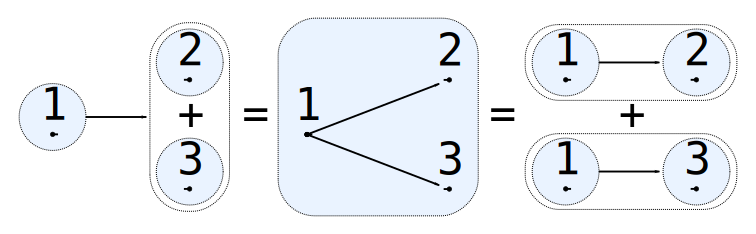
\includegraphics[scale=0.27]{fig/ax-distributivity.pdf}}
\caption{Distributivity: $1 \rightarrow (2 + 3) = 1 \rightarrow 2 + 1 \rightarrow 3$ }
\end{subfigure}
\hspace{12mm}
\begin{subfigure}[b]{0.5\linewidth}
\centerline{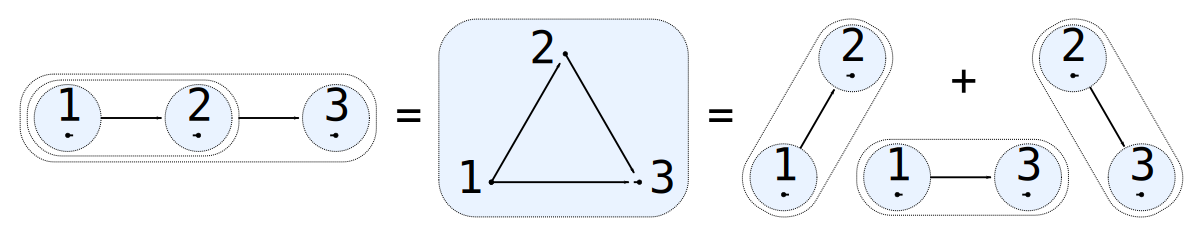
\includegraphics[scale=0.27]{fig/ax-decomposition.pdf}}
\caption{Decomposition: $1 \rightarrow 2 \rightarrow 3 = 1 \rightarrow 2 +
1 \rightarrow 3 + 2 \rightarrow 3$}
\end{subfigure}
\caption{Two axioms of the algebra of graphs.\label{fig-axioms}}
\end{figure*}

\section{Algebraic structure}\label{sec-algebra}

The functions \hs{edge}, \hs{vertices} and \hs{clique} defined in the previous
section \S\ref{sec-core} satisfy a few properties that we can intuitively write down
and verify at the level of sets of vertices and edges:
\begin{itemize}
    \item \hs{vertex@\,\blk{x}@} $\ =\ $ \hs{vertices@\,@[x]} and
    \hs{edge@\,\blk{x}\,\blk{y}@} $\ =\ $ \hs{clique@\,@[x,y]}.
    \item \hs{vertices xs} $\ \subseteq\ $ \hs{clique xs}, where $x \subseteq y$ means
    $x$ is a \emph{subgraph} of $y$, i.e. $V_x\subseteq V_y$ and $E_x\subseteq E_y$ hold.
    \item \hs{clique@\,@(xs@\,@++@\,\blk{ys}@)} $\ =\ $ \hs{connect@\,@(}\hs{clique@\,\blk{xs}@)@\,@(}\hs{clique@\,\blk{ys}@)}.
\end{itemize}

In this section we characterise the \hs{Graph} type class with a set of
axioms that reveal an algebraic structure very similar to a semiring\footnote{
See~\citet{1999_semirings_golan} for a classic overview of semiring
applications, where the author hints at the existence of a non-semiring `algebra of
digraphs' whose operations coincide with overlay and connect, referring to an unpublished
paper by Anthony P. Stone. \citet{2013_semirings_dolan} uses the semiring theory to
implement graph algorithms.}.
This provides a convenient framework for proving graph properties, such as
those listed above, using equational reasoning. The presented characterisation is
generally useful for formal verification, as well as automated testing of graph library
APIs.

\subsection{Axiomatic characterisation}\label{sub-laws}

The definitions of \hs{vertices} and \hs{clique} in \S\ref{sub-class}
use $\varepsilon$ as the identity for both overlay $+$ and connect $\rightarrow$
operations. This seems unusual, but we can check that
$x + \varepsilon = x$ and $x \rightarrow \varepsilon = x$ for any graph $x \in G$
by plugging the empty graph into the definitions of overlay and connect,
respectively. Furthermore, we can verify the following:
\begin{itemize}
    \item $(G,+,\varepsilon)$ is an idempotent commutative monoid.
    \item $(G,\rightarrow,\varepsilon)$ is a monoid.
    \item $\rightarrow$ distributes over $+$, as illustrated
    in Fig.~\ref{fig-axioms}(a).
\end{itemize}

\noindent
The above looks remarkably close to a semiring, with the only oddity being the shared
identity of the two operations. The lack of annihilating zero element and the
following \emph{decomposition} law is what makes the algebra of graphs different:
\[
x \rightarrow y \rightarrow z = x \rightarrow y + x \rightarrow z + y \rightarrow z.
\]

\noindent
Fig.~\ref{fig-axioms}(b) illustrates the law by showing that the triangle
graph can be obtained in two different ways: by connecting the three vertices
of the triangle or by constructing its edges separately and overlaying them.

Interestingly, the fact that overlay and connect share the same identity
follows from the decomposition law. Indeed, let $\varepsilon_{+}$ and
$\varepsilon_{\rightarrow}$ stand for the identities of $+$ and $\rightarrow$,
respectively. Then:
\[
\begin{array}{rcll}
\varepsilon_{+} & = & \varepsilon_{+} \rightarrow \varepsilon_{\rightarrow} \rightarrow \varepsilon_{\rightarrow} & \text{(identity of $\rightarrow$)}\\
 & = & \varepsilon_{+} \rightarrow \varepsilon_{\rightarrow} + \varepsilon_{+} \rightarrow \varepsilon_{\rightarrow} + \varepsilon_{\rightarrow} \rightarrow \varepsilon_{\rightarrow} & \text{(decomposition)}\\
 & = & \varepsilon_{+} + \varepsilon_{+} + \varepsilon_{\rightarrow} & \text{(identity of $\rightarrow$)}\\
 & = & \varepsilon_{\rightarrow} & \text{(identity of $+$)}\\
\end{array}
\]

\noindent
Furthermore, the idempotence of $+$ can also be proved from the decomposition, which
leads to the following \emph{minimal set of axioms that characterise algebraic graphs}.

\begin{itemize}
    \item $+$ is commutative and associative, i.e. $x + y = y + x$ and
    $x + (y + z) = (x + y) + z$.
    \item $(G, \rightarrow, \varepsilon)$ is a monoid, i.e.
    $\varepsilon \rightarrow x = x$, $x \rightarrow \varepsilon = x$ and
    $x \rightarrow (y \rightarrow z) = (x \rightarrow y) \rightarrow z$.
    \item $\rightarrow$ distributes over $+$:
    $x \rightarrow (y + z) = x \rightarrow y + x \rightarrow z$ and
    $(x + y) \rightarrow z = x \rightarrow z + y \rightarrow z$.
    \item Decomposition: $x \rightarrow y \rightarrow z =
    x \rightarrow y + x \rightarrow z + y \rightarrow z$.
\end{itemize}

We require all \hs{Graph} instances to satisfy these 8 axioms. Our definition
of graph construction primitives in~\S\ref{sub-constructing} does satisfy them
all and is therefore a valid \hs{Graph} instance. We will provide an
implementation for this and other useful instances in~\S\ref{sec-a-la-carte}.
Some of them will satisfy additional
axioms; for example, by making the connect operation commutative,
we obtain undirected graphs.

Algebraic graphs are \emph{complete} in the sense that it is possible to describe
any graph using the core interface. Indeed, given a graph $(V,E)$ we can construct
it as \hs{graph@$\,V\,E$@}, where the function \hs{graph} is defined as follows.

\begin{minted}{haskell}
graph :: Graph g@\,@=>@\,@[Vertex g]@\,@->@\,@[(Vertex g,@\,@Vertex g)]@\,@->@\,\blk{g}@
graph vs es = overlay (vertices vs) (edges es)
\end{minted}

Here \hs{edges} is a generalisation of the function \hs{edge} to a list of edges,
so that \hs{edge x y} $\ =\ $ \hs{edges [(x,y)]}:

\begin{minted}{haskell}
edges :: Graph g => [(Vertex g, Vertex g)] -> g
edges = @\std{foldr}@ overlay empty . @\std{map}@ (@\std{uncurry}@ edge)
\end{minted}

The \emph{absorption theorem} $x \rightarrow y + x + y = x \rightarrow y$, which
follows from decomposition of $x \rightarrow y \rightarrow \varepsilon$, states
that an edge $(u,v)$ contains its two vertices $\{u,v\}$ and is inseparable from
them. Therefore, if the pair $(V,E)$ is inconsistent, the set of vertices of
\hs{graph@$\,V\,E$@} will be expanded to $\hat{V}$ so that
$E\subseteq \hat{V}\times \hat{V}$ holds. More generally, the absorption
theorem states that in addition to being complete, the algebraic graph
API is also \emph{sound} in the sense that it is impossible to construct
an inconsistent pair $(V,E)$ using the four \hs{Graph} methods.

The following theorems can be proved from the axioms:

\begin{itemize}
    \item Identity of $+$: $x + \varepsilon = x$.
    \item Idempotence of $+$: $x + x = x$.
    \item Absorption: $x \rightarrow y + x + y = x \rightarrow y$.
    \item Saturation: $x \rightarrow x \rightarrow x = x \rightarrow x$.
\end{itemize}

These theorems were proved in Agda by~\citet{2014_alekseyev_phd} who formalised
the algebra of parameterised graphs that we build on.

\begin{figure*}
\[
\begin{array}{rcll}
\hspace{6mm}\hs{vertices (h:t)} & = & \hs{@\std{foldr}@ overlay empty (@\std{map}@ vertex (h:t))} & \text{(definition of \hs{vertices})}\\
 & = & \hs{@\std{foldr}@ overlay empty (vertex h : @\std{map}@ vertex t)} & \text{(definition of }\hs{@\std{map}@}\text{)}\\
 & = & \hs{overlay (vertex h) (vertices t)} & \text{(definition of }\hs{@\std{foldr}@}\text{)}\\
 & \subseteq & \hs{overlay (vertex h) (clique t)} & \text{(monotony and the inductive hypothesis)}\\
 & \subseteq & \hs{connect (vertex h) (clique t)} & \text{(overlay-connect order)}\\
 & = & \hs{@\std{foldr}@ connect empty (vertex h : @\std{map}@ vertex t)} & \text{(definition of }\hs{@\std{foldr}@}\text{)}\\
 & = & \hs{@\std{foldr}@ connect empty (@\std{map}@ vertex (h:t))} & \text{(definition of }\hs{@\std{map}@}\text{)}\\
 & = & \hs{clique (h:t)} & \text{(definition of \hs{clique})}\\
\end{array}
\]
\caption{Equational reasoning with algebraic graphs.\label{fig-proof}}
\end{figure*}

\subsection{Partial order on graphs}\label{sub-partial-order}

It is fairly standard to define $x \preceq y$ as $x + y = y$ for an
idempotent operation~$+$, since it gives a partial order on the elements
of the algebra. Indeed, all partial order laws are satisfied:

\begin{itemize}
     \item Reflexivity $x \preceq x$ follows from the idempotence $x + x = x$.
     \item Antisymmetry $x \preceq y \wedge y \preceq x \Rightarrow x = y$ holds
     since $x + y = y$ and $y + x = x$ imply $x = y$.
     \item Transitivity $x \preceq y \wedge y \preceq z \Rightarrow x \preceq z$
     can be proved as $z = y + z = (x + y) + z = x + (y + z) = x + z$.
 \end{itemize}

\noindent
It turns out that this definition corresponds to the \emph{subgraph} relation,
i.e. we can define:
\[
x \subseteq y~~\defeq~~x + y = y.
\]

\noindent
Indeed, expanding $x + y = y$ to $(V_x,E_x) + (V_y,E_y) = (V_y,E_y)$ gives us
$V_x \cup V_y = V_y$ and $E_x \cup E_y = E_y$, which is equivalent to
$V_x \subseteq V_y$ and $E_x \subseteq E_y$, as desired.

Therefore, we can check if a graph is a subgraph of another one if we know how to
compare graphs for equality:
\begin{minted}{haskell}
isSubgraphOf :: (Graph g, Eq g) => g -> g -> Bool
isSubgraphOf x y = overlay x y == y
\end{minted}

The following theorems about the partial order on graphs can be proved:

\begin{itemize}
    \item Least element: $\varepsilon \subseteq x$.
    \item Overlay order: $x \subseteq x + y$.
    \item Overlay-connect order: $x + y \subseteq x \rightarrow y$.
    \item Monotony: $x \subseteq y \Rightarrow \\
    (x + z \subseteq y + z) \wedge(x \rightarrow z \subseteq y \rightarrow z)
    \wedge (z \rightarrow x \subseteq z \rightarrow y)$.

\end{itemize}

\subsection{Equational reasoning}\label{sub-reasoning}

In this subsection we show how to use equational reasoning and the laws
of the algebra to prove properties of functions on graphs.
For example, to prove that \hs{vertex x} $=$ \hs{vertices [x]} we rewrite
the right-hand side using the function definitions and $x + \varepsilon = x$:
\[
\begin{array}{rcl}
\hs{vertices [x]} & = & \hs{@\std{foldr}@ overlay empty (@\std{map}@ vertex [x])}\\
 & = & \hs{@\std{foldr}@ overlay empty [vertex x]}\\
 & = & \hs{overlay (vertex x) empty}\\
 & = & \hs{vertex x}\\
\end{array}
\]

Proving that \hs{vertices xs} $\ \subseteq\ $ \hs{clique xs} requires more work.
We start with the case when $\hs{@\blk{xs}@}$ is the empty list $\hs{[@@]}$,
which is straightforward:
$\hs{vertices [@@]} = \varepsilon \subseteq \varepsilon = \hs{clique [@@]}$,
as follows from the definition of \hs{@\std{foldr}@}.
If $\hs{@\blk{xs}@}$ is non-empty, i.e. $\hs{@\blk{xs}@}\ =\ \hs{@\blk{h}@:t}$,
we make the inductive hypothesis that
\hs{vertices t} $\ \subseteq\ $ \hs{clique t} and proceed as shown in Fig.~\ref{fig-proof}.

% \begin{figure}[b]
% \vspace{-2mm}
% \begin{subfigure}[b]{0.48\linewidth}
% \begin{minted}{haskell}
% gen ::@\,@(Graph g,@\,@Arbitrary@\,@(Vertex g)) => Gen g
% gen = sized expr
%   where
%     expr 0 = @\std{return}@ empty
%     expr 1 = @\std{fmap}@ vertex arbitrary
%     expr n = do
%         sizeLeft <- choose (0, n)
%         l <- expr sizeLeft
%         r <- expr (n - sizeLeft)
%         elements [ overlay l r, connect l r ]

% instance Arbitrary a => Arbitrary@\,@(Expr@\,@a) where
%     arbitrary = gen

%     shrink Empty = []
%     ...
% \end{minted}
% \caption{Generating arbitrary algebraic graphs}
% \end{subfigure}
% \hfill
% \hfill
% \hfill
% \vrule
% \hfill
% \begin{subfigure}[b]{0.45\linewidth}
% \begin{minted}{haskell}
% (+) = overlay -- convenient shortcuts
% (*) = connect

% type GraphTestsuite g = (Eq g, Graph g)
%   => g -> g -> g -> Property

% axioms :: GraphTestsuite g
% axioms x y z = conjoin
%   [       x + y == y + x
%   , x + (y + z) == (x + y) + z
%   ,   empty * x == x
%   ,   x * empty == x
%   , x * (y * z) == (x * y) * z
%   , x * (y + z) == x * y + x * z
%   , (x + y) * z == x * z + y * z
%   ,   x * y * z == x * y + x * z + y * z ]
% \end{minted}
% \caption{Testsuite for the minimal set of axioms}
% \end{subfigure}
% \vspace{-3mm}
% \caption{Automated testing infrastructure for algebraic graphs\label{fig-testing}}
% \end{figure}

% \subsection{Automated testing}\label{sub-testing}

% Theorem provers, such as Agda~\cite{2007_norell_agda},
% can substantially reduce the effort required for formal verification,
% however, automated testing remains an effective and pervasively used
% method for formulating and testing functional properties. In Haskell,
% the go-to tool for automated testing is QuickCheck developed
% by~\citet{2011_quickcheck_claessen}.
% Fig.~\ref{fig-testing} shows a reusable testing infrastructure for
% algebraic graphs. The function~\hs{gen} in Fig.~\ref{fig-testing}(a)
% allows to generate arbitrary graph expressions of specified size.
% It is polymorphic and can therefore be used as a default implementation
% of QuickCheck's \hs{Arbitrary} type class, as shown by a sketch of
% the \hs{Arbitrary@\,\,@(Expr@\,\,\blk{a}@)} instance definition, where \hs{Expr}
% is a \hs{Graph} instance defined in the next section~\S\ref{sec-a-la-carte}.

% Fig.~\ref{fig-testing}(b) shows an implementation of the \hs{axioms}
% testsuite that can be used for testing a \hs{Graph} instance against
% the minimal set of axioms defined in~\S\ref{sub-laws}.
% For example, let's do a quick check of \hs{Expr@\,@Int} in the interactive GHC:

% \begin{minted}[frame=single]{haskell}
% @\ghci @quickCheck (axioms :: GraphTestsuite (Expr Int))
% @\blk{+++ OK, passed 100 tests.}@
% \end{minted}

% \noindent
% Here QuickCheck generates 100 random test cases $(x,y,z)$ using the \hs{gen}
% function and checks that \hs{axioms@\,$x\,y\,z$@} holds in each case. Note
% that we have to tell QuickCheck which specific \hs{Graph} instance to test
% by providing a type signature for the polymorphic \hs{axioms} testsuite.

% Finally, let's use QuickCheck to test the property
% \hs{clique (xs ++ ys)} $\ =\ $ \hs{connect (}\hs{clique xs) (}\hs{clique ys)},
% which we contemplated in the beginning of this section:

% \begin{minted}[frame=single]{haskell}
% @\ghci @quickCheck $ \xs ys -> clique@\,@(xs ++ ys) == connect@\,@(clique xs) (clique ys :: Epxr Int)
% @\blk{+++ OK, passed 100 tests.}@
% \end{minted}

% \noindent
All properties and theorems that we discuss in this paper have been
formally proved in Agda\footnote{The proofs are available at
\url{https://github.com/snowleopard/alga-theory}.}.

%!TEX root = alga.tex
\section{Graphs \`{a} la carte}\label{sec-a-la-carte}

In this section we define several useful \hs{Graph} instances, and
show that the algebra presented in the previous section~\S\ref{sec-algebra} is
not restricted only
to directed graphs, but can be extended to axiomatically represent undirected,
reflexive, transitively closed, and labelled graphs, their various
combinations, and even hypergraphs.

\begin{figure}[b]
\vspace{-3mm}
\begin{minted}{haskell}
import           Data.Set (Set, @\blk{singleton, union, elems, fromAscList}@)
import qualified Data.Set as Set (empty)
\end{minted}
\vspace{1mm}
\begin{minted}{haskell}
data Relation a = Relation { domain :: Set a, relation :: Set (a, a) } deriving (Eq, Show)
\end{minted}
\vspace{1mm}
\begin{minted}{haskell}
instance Ord a => Graph (Relation a) where
    type Vertex (Relation a) = a
    empty       = Relation Set.empty Set.empty
    vertex  x   = Relation (singleton x) Set.empty
    overlay x y = Relation (domain x `union` domain y) (relation x `union` relation y)
    connect x y = Relation (domain x `union` domain y) (relation x `union` relation y
        `union` fromAscList [ (a, b) | a <- elems (domain x), b <- elems (domain y) ])
\end{minted}
\vspace{-3mm}
\caption{Implementing the \hs{Graph} type class by a binary relation
and the core graph construction primitives
defined in~\S\ref{sub-constructing}\label{fig-relation}}
\vspace{-3mm}
\end{figure}

\subsection{Binary relation}\label{sub-relation}

We start by a direct encoding of the graph construction primitives defined
in~\S\ref{sub-constructing} into the \hs{Relation} data type isomorphic
to a pair of sets $(V,E)$, see Fig.~\ref{fig-relation}. As we have seen,
this implementation satisfies the axioms of the graph algebra. Furthermore, it
is a \emph{free graph} in the sense that it does not satisfy any other laws.
This follows from the fact that any algebraic graph expression $g$ can be
rewritten in the following \emph{canonical form}:
\[
g = \Big(\sum_{v\in V_g} v\Big) + \Big(\sum_{(u,v)\in E_g} \hspace{-1mm} u \rightarrow v\Big),
\]
\vspace{-1mm}
\noindent
where $V_g$ is the set of vertices that appear in $g$, and $(u,v)\in E_g$ if
vertices $u$ and $v$ appear in the left-hand and right-hand arguments of
the connect operation $\rightarrow$ at least once (and should thus be connected
by an edge). The canonical form of an
expression $g$ can be represented as \hs{Relation@$\,\,V_g\,E_g$@},
and any additional law on \hs{Relation} would violate the canonicity property.
The existence of the canonical form has been proved by~\citet{2014_algebra_mokhov}
for an extended version of the algebra. The proof fundamentally builds on the
decomposition axiom: one can apply it repeatedly to an expression, breaking up
connect sequences $x\rightarrow y\rightarrow z$ into pairs $x \rightarrow y$
until the decomposition can no longer be applied. We can then open the parentheses
using the distributivity and rearrange terms into the canonical expression
by the commutativity and idempotence of the overlay $+$ operation.

It is convenient to make \hs{Relation} an instance of the \hs{Num} type class
to use the standard $+$ and $*$ operators as shortcuts for \hs{overlay} and
\hs{connect}, respectively:

\begin{minted}{haskell}
instance (Ord a, Num a) => Num (Relation a) where
    fromInteger = vertex . fromInteger
    (+)         = overlay
    (*)         = connect
    signum      = const empty
    abs         = id
    negate      = id
\end{minted}

\noindent
Note that the \hs{Num} law \hs{@\blk{abs}@ x * signum x == x} is satisfied by the above
definition since $x \rightarrow \varepsilon = x$. In fact, any \hs{Graph} instance
can be made a law-abiding \hs{Num} instance if need be, using a definition similar to the above.

We can now play with graphs and binary relations using the interactive GHC:

\begin{minted}[frame=single]{haskell}
@\ghci@ 1 * (2 + 3) :: Relation Int
Relation {domain = fromList [1,2,3], relation = fromList [(1,2),(1,3)]}
@\ghci@ 1 * (2 + 3) + 2 * 3 == (clique [1..3] :: Relation Int)
True
@\ghci@ 1 * 2 == (2 * 1 :: Relation Int)
False
@\ghci \blk{:t}@ clique "abcd"
clique "abcd" :: (Graph g, Vertex g @\teq@ Char) => g
@\ghci @relation (clique "abcd")
fromList [('a','b'),('a','c'),('a','d'),('b','c'),('b','d'),('c','d')]
\end{minted}

\noindent
The last example highlights the fact that the \hs{Relation@\,\,\blk{a}@} instance allows vertices
of any type \hs{@\blk{a}@} that satisfies the~\hs{Ord@\,\,\blk{a}@} constraint.

\subsection{Deep embedding}\label{sub-embedding}

By embedding the core graph construction primitives into a basic algebraic data type
we obtain the following simple \hs{Graph} instance:

\begin{minted}{haskell}
data Expr a = Empty | Vertex a | Overlay (Expr a) (Expr a) | Connect (Expr a) (Expr a)
    deriving Show

instance Graph (Expr a) where
    type Vertex (Expr a) = a
    empty   = Empty
    vertex  = Vertex
    overlay = Overlay
    connect = Connect
\end{minted}

The instance definition provides a mapping from the \emph{shallow embedding}
of the core primitives, represented by the type class \hs{Graph}, into the
corresponding \emph{deep embedding}, represented by the data type \hs{Expr}.
It is known, e.g. see~\citet{2014_gibbons_folding}, that by \emph{folding} the data
type one can always obtain the inverse mapping:

\begin{minted}{haskell}
fold :: (Graph g, Vertex g @\teq@ a) => Expr a -> g
fold Empty         = empty
fold (Vertex  x  ) = vertex x
fold (Overlay x y) = overlay (fold x) (fold y)
fold (Connect x y) = connect (fold x) (fold y)
\end{minted}

We cannot use the derived \hs{Eq} instance of the \hs{Expr} data type, because it
would clearly violate the axioms of the algebra, e.g. \hs{Overlay@\,\,@Empty@\,\,@Empty} is
structurally different from \hs{Empty}, but they must be equal according to the axioms.
However, we can implement a custom law-abiding \hs{Eq}
instance by \emph{reinterpreting} the graph expression \hs{Expr}
as a \hs{Relation}, thereby gaining access to the canonical graph representation:

\begin{minted}{haskell}
instance Ord a => Eq (Expr a) where
    x == y = fold x == (fold y :: Relation a)
\end{minted}

An interesting feature of the \hs{Expr} instance is that it allows to represent
densely connected graphs more compactly. For example, \hs{clique [1..n] :: Expr Int}
has a linear-size representation in memory, while \hs{clique [1..n] :: Relation Int}
stores each edge separately and therefore uses $O(n^2)$ memory. Exploiting the
compact graph representation for deriving algorithms that are asymptotically faster
on dense graphs, compared to conventional algorithms operating on `uncompressed'
graph representations isomorphic to $(V,E)$, is outside the scope of this paper,
but is an interesting direction of future research.

\begin{figure}[b]
\vspace{-2mm}
\begin{minted}{haskell}
import           Data.Map.Strict (Map, keysSet, fromSet)
import qualified Data.Map.Strict as Map
import           Data.Set (Set)
import qualified Data.Set as Set
\end{minted}
\vspace{1mm}
\begin{minted}{haskell}
newtype AdjacencyMap a = AM { adjacencyMap :: Map a@\,\,@(Set a) }@\,\,@deriving@\,\,@(Arbitrary,@\,\,@Eq,@\,\,@Show)
\end{minted}
\vspace{1mm}
\begin{minted}{haskell}
instance Ord a => Graph (AdjacencyMap a) where
    type Vertex (AdjacencyMap a) = a
    empty       = AM $ Map.empty
    vertex  x   = AM $ Map.singleton x Set.empty
    overlay x y = AM $ Map.unionWith Set.union (adjacencyMap x) (adjacencyMap y)
    connect x y = AM $ Map.unionsWith Set.union [ adjacencyMap x, adjacencyMap y,
        fromSet (const . keysSet $ adjacencyMap y) (keysSet $ adjacencyMap x) ]
\end{minted}
\vspace{-3mm}
\caption{Implementing the \hs{Graph} type class by adjacency map\label{fig-adjacency-map}}
\vspace{-1mm}
\end{figure}

\subsection{Adjacency map and topological sort}\label{sub-adjacency-map}

In this subsection we show how to reuse existing graph libraries, such as
\textsf{containers} and \textsf{fgl}, by wrapping them into the algebraic
graph API. More specifically, we show how to reuse the efficient implementation of
the \emph{topological sort} algorithm developed by~\citet{1995_king_graphs}.

The interface of the \textsf{containers} library uses the \emph{adjacency list}
representation of graphs and we therefore define a new \hs{Graph} instance that
provides the closest match, see Fig.~\ref{fig-adjacency-map}. In our experiments
this instance is often faster than \hs{Relation} because of more efficient
sharing of common subgraphs in memory, see~\S\ref{sub-benchmarks}.

The \hs{AdjacencyMap} instance is parametric and in order to use the
functions provided by \textsf{containers}, we need to map the graph vertices
into contiguous subsets of integers \hs{Int}. This can be done by the function
\hs{graphFromEdges} defined in \textsf{containers} that requires an adjacency list as
the input. We can obtain the adjacency list from \hs{AdjacencyMap} as follows:

\begin{minted}{haskell}
adjacencyList :: AdjacencyMap a -> [(a, [a])]
adjacencyList = @\std{map}@ (@\std{fmap}@ Set.toAscList) . Map.toAscList . adjacencyMap
\end{minted}
Both \textsf{containers} and \textsf{fgl} also provide graph constructors from the
\emph{edge list} graph representation, which can be readily obtained from
\hs{adjacencyList}:

\begin{minted}{haskell}
edgeList :: AdjacencyMap a -> [(a, a)]
edgeList = concatMap (\(x, ys) -> @\std{map}@ (x,) ys) . adjacencyList
\end{minted}

\noindent
Let's test that \hs{AdjacencyMap} is a valid \hs{Graph} instance and
showcase \hs{adjacencyList} and \hs{edgeList}:

\begin{minted}[frame=single]{haskell}
@\ghci @quickCheck (axioms :: GraphTestsuite (AdjacencyMap Int))
@\blk{+++ OK, passed 100 tests.}@

@\ghci @adjacencyList $ clique [1..4]
[(1,[2,3,4]),(2,[3,4]),(3,[4]),(4,[@@])]

@\ghci @edgeList $ edges [('a','b'),('b','c'),('a','b')]
[('a','b'),('b','c')]
\end{minted}

We can now build safe bridges to \textsf{containers} and \textsf{fgl}. Consider
the following wrapper\footnote{We use \textsf{GeneralizedNewtypeDeriving} GHC
extension to derive \hs{Arbitrary}, \hs{Graph} and \hs{Num} instances. Note that
the current version of GHC does not support the extension for classes
with associated types, such as \hs{Graph}, but the feature has already been
implemented and will be available in the next GHC release. Until then
one needs to write the trivial \hs{Graph} instance manually.}
around \hs{AdjacencyMap}:

\begin{minted}{haskell}
newtype TopSort a = TS (AdjacencyMap a) deriving (Arbitrary, Graph, Num, Show)
\end{minted}
\vspace{1mm}
\begin{minted}{haskell}
instance Ord a => Eq (TopSort a) where
    x == y = topSort x == topSort y
\end{minted}
\vspace{1mm}
\begin{minted}{haskell}
topSort :: Ord a => TopSort a -> Maybe [a]
topSort = ... -- call Data.Graph.topSort via Data.Graph.graphFromEdges
\end{minted}

\noindent
The \hs{TopSort} instance differs from \hs{AdjacencyMap} only in one aspect: it uses
a custom equality test, which satisfies more laws than required by the \hs{Graph}
instance. Indeed, there are many pairs of different graphs, whose topological sorts
coincide, e.g. \hs{topSort (1 + 2)} = \hs{topSort (1 * 2)} = \hs{Just [1,2]}.

We do not show the implementation of the \hs{topSort} function here, as it is not
particularly interesting and involves low-level plumbing, however we would like to
emphasise that the resulting interface is fully parametric and safe. Note the
return type of \hs{topSort}: the function returns \hs{Nothing}
if a topological sort does not exist because the graph is cyclic; otherwise it
returns a list of vertices in the topological order, as demonstrated below:

\begin{minted}[frame=single]{haskell}
@\ghci @quickCheck (axioms :: GraphTestsuite (TopSort Int))
@\blk{+++ OK, passed 100 tests.}@

@\ghci @topSort $ 1 * 2 + 3 * 1
Just [3,1,2]

@\ghci @topSort $ 1 * 2 + 2 * 1
Nothing
\end{minted}

\subsection{Undirected graphs}\label{sub-undirected}

As hinted in \S\ref{sub-laws}, to switch from directed to undirected graphs it
is sufficient to add the axiom of commutativity for the connect operator. For
undirected graphs it makes sense to denote the connect operation by $\leftrightarrow$ or
\textemdash, hence:

\begin{itemize}
    \item $\leftrightarrow$ is commutative: $x \leftrightarrow y = y \leftrightarrow x$.
\end{itemize}

Curiously, with the introduction of this axiom, the associativity of $\leftrightarrow$
follows from the left-associated version of the decomposition axiom and the
commutativity of $+$:
\[
\begin{array}{rcll}
(x \leftrightarrow y) \leftrightarrow z & = & x \leftrightarrow y + x \leftrightarrow z + y \leftrightarrow z & \text{(left decomposition)}\\
 & = & y \leftrightarrow z + y \leftrightarrow x + z \leftrightarrow x & \text{(commutativity of $+$ and $\leftrightarrow$)}\\
 & = &  (y \leftrightarrow z) \leftrightarrow x & \text{(left decomposition)}\\
 & = &   x \leftrightarrow (y \leftrightarrow z) & \text{(commutativity of $\leftrightarrow$)}\\
\end{array}
\]

Therefore, \emph{the minimal set of axioms of undirected graphs} comprises only 6 axioms:

\begin{itemize}
    \item $+$ is commutative and associative: $x + y = y + x$ and
    $x + (y + z) = (x + y) + z$.
    \item $\leftrightarrow$ is commutative $x \leftrightarrow y = y \leftrightarrow x$ and
    has $\varepsilon$ is the identity: $x \leftrightarrow \varepsilon = x$.
    \item Distributivity:
    $x \leftrightarrow (y + z) = x \leftrightarrow y + x \leftrightarrow z$.
    \item Left decomposition: $(x \leftrightarrow y) \leftrightarrow z =
    x \leftrightarrow y + x \leftrightarrow z + y \leftrightarrow z$.
\end{itemize}

Commutativity of the connect operator forces graph expressions that differ only
in the direction of edges into the same equivalence class. One can implement
this by the \emph{symmetric closure} of the underlying relation:

\begin{minted}{haskell}
newtype Undirected a = U (Relation a) deriving (Arbitrary, Graph, Num, Show)

instance Ord a => Eq (Undirected a) where
    U x == U y = symmetricClosure x == symmetricClosure y

symmetricClosure :: Ord a => Relation a -> Relation a
symmetricClosure = ... -- direct edges canonically or make them bidirectional
\end{minted}

Note that algebraic expressions of undirected graphs have the canonical form where all
edges are directed in a canonical order, e.g. according to some total order on vertices.

Let's test that the custom equality works as desired:
\begin{minted}[frame=single]{haskell}
@\ghci @quickCheck (axioms :: GraphTestsuite (Undirected Int))
+++ OK, passed 100 tests.

@\ghci @quickCheck $ \x y -> x * y == (y * x :: Undirected Int)
+++ OK, passed 100 tests.

@\ghci @clique "abcd" == (clique "dcba" :: Relation Char)
False

@\ghci @clique "abcd" == (clique "dcba" :: Undirected Char)
True
\end{minted}

As you can see, the polymorphic graph construction functions, such as \hs{clique},
can be safely used when working with undirected graphs. We can define a subclass
\hs{class Graph g => UndirectedGraph g} and use the \hs{UndirectedGraph g}
constraint for functions that rely on the commutativity of the \hs{connect} method.

\subsection{Reflexive and irreflexive graphs}

A graph is \emph{reflexive} if every vertex is connected to itself, i.e. has a self-loop.
An example of a reflexive graph is the graph corresponding to the partial
order relation $\subseteq$ on graphs: indeed, $x \subseteq x$ holds for all $x$. To
represent reflexive graphs algebraically we can introduce the following axiom:

\begin{itemize}
    \item $v = v \rightarrow v$, where $v\in \mathbb{V}$ is a vertex.
\end{itemize}

\noindent
The axiom corresponds to an additional \hs{Graph} type class law:
\hs{vertex x} = \hs{connect (}\hs{vertex x) (}\hs{vertex x)}.

One way to look at the axiom is that it enforces that each vertex has a self-loop. However,
there is another equally valid perspective, which corresponds to the reverse application
of the equality, wherein the axiom states that there are no self-loops! This may seem like an
internal contradiction of the theory, but in fact this simply indicates the isomorphism
between reflexive and \emph{irreflexive} graphs: you can always
turn a reflexive graph into the corresponding irreflexive one by deleting the self-loops,
and vice versa.

One can implement the reflexive and/or irreflexive \hs{Graph} instance very similarly to
the \hs{Undirected} implementation presented in~\S\ref{sub-undirected}: simply wrap
\hs{Relation} into a \hs{newtype} and give it a custom \hs{Eq} instance based on the
\hs{reflexiveClosure}.

We can define
\hs{class Graph g => ReflexiveGraph g} and \hs{class Graph g => IrreflexiveGraph g}
to increase the type safety of functions that rely on the additional axiom. It seems
strange to have two different type classes with exactly the same methods and laws, but
it may be useful to distinguish their semantics.

\subsection{Transitively closed graphs}

In many applications graphs satisfy the \emph{transitivity} property: if a vertex $x$ is
connected to $y$, and $y$ is connected to $z$, then the edge between $x$ and $z$ can be
added or removed without changing the semantics of the graph. A common example is
\emph{dependency graphs} or \emph{partial orders} --- the semantics of such graphs is
typically their \emph{transitive closure}.
To describe this class of graphs algebraically we add the following \emph{closure} axiom:

\begin{itemize}
    \item Closure: $y \neq \varepsilon \Rightarrow x \rightarrow y + y \rightarrow z +
    x \rightarrow z = x \rightarrow y + y \rightarrow z$.
\end{itemize}

By using the axiom one can rewrite a graph expression into its transitive closure or,
alternatively, into its \emph{transitive reduction}, hence all graphs that differ only in the
existence of some transitive edges are forced into the same equivalence class. Note that the
precondition $y \neq \varepsilon$ is necessary as otherwise $+$ and $\rightarrow$ can no
longer be distinguished:
\[
x \rightarrow z = x \rightarrow \varepsilon \rightarrow z = x \rightarrow \varepsilon
 + \varepsilon \rightarrow z + x \rightarrow z = x \rightarrow \varepsilon
 + \varepsilon \rightarrow z = x + z.
\]

It is interesting to note that $+$ and $\rightarrow$ have a simple meaning for transitively
closed graphs: they correspond to the \emph{parallel} and \emph{sequential composition},
respectively. This allows to algebraically describe concurrent systems, which was one
of the original motivations behind the research on algebraic graphs.

We can implement a \hs{Graph} instance for transitively closed graphs by wrapping
\hs{Relation} in a \hs{newtype} with a custom equality function, which given two
graphs compares the transitive closures of the underlying relations.

The above implementation permits cycles in graphs, therefore the resulting equivalence
classes correspond to \emph{preorders}. For example, $(1 + 2 + 3) \rightarrow (2 + 3 + 4)$
is a preorder with vertices 2 and 3 forming a \emph{strongly-connected component}. By
finding all strongly-connected components in the graph (e.g. by using the function \hs{scc}
from the \textsf{containers} library) we can derive the following \emph{graph condensation}:
$\{1\} \rightarrow \{2, 3\} \rightarrow \{4\}$. One way to interpret this preorder as a
dependency graph is that tasks 2 and 3 are executed as a step,
simultaneously, and that they both depend on task 1, and are required for task 4.

A subclass \hs{class Graph g => TransitiveGraph g} can be defined to distinguish
algebraic graphs with the closure axiom from others.

\subsection{Hypergraphs}

As described in~\S\ref{sub-relation}, the decomposition axiom collapses an algebraic
graph expression into a collection of vertices and pairs of vertices, i.e. graphs. By replacing
the decomposition axiom with \emph{3-decomposition}, we obtain \emph{hypergraphs} comprising
vertices, edges and \emph{3-edges} (triples of vertices):

\begin{itemize}
    \item 3-decomposition: $w \rightarrow x \rightarrow y \rightarrow z =
    w \rightarrow x \rightarrow y + w \rightarrow x \rightarrow z +
    w \rightarrow y \rightarrow z + x \rightarrow y \rightarrow z$.
\end{itemize}

To better understand the difference between the (2-)decomposition and 3-decomposition
axioms, let's substitute~$\varepsilon$ for $w$ in the 3-decomposition and simplify:
\[
x \rightarrow y \rightarrow z = x \rightarrow y + x \rightarrow z + y \rightarrow z
+ x \rightarrow y \rightarrow z.
\]
Looks familiar? This is almost the 2-decomposition axiom! Yet there is no way to get rid
of the term $x \rightarrow y \rightarrow z$ on the right-hand side: indeed, a triple is
unbreakable
in this algebra, and one can only extract the pairs (edges) that are embedded in it.
In fact, we can take this further and rewrite the above expression to also expose the
embedded vertices:
\[
x \rightarrow y \rightarrow z = x + y + z + x \rightarrow y + x \rightarrow z
+ y \rightarrow z + x \rightarrow y \rightarrow z.
\]
Note that with 2-decomposition we can achieve something similar via the absorption theorem:
\[
x \rightarrow y = x + y + x \rightarrow y.
\]
This can be taken further by defining 4-decomposition and so forth, creating a hierarchy
of algebraic structures.

Since every graph is also a hypergraph, we can define a superclass
\hs{class HyperGraph g => Graph g}, moving all \hs{Graph} methods to the superclass, and
leaving only the decomposition axiom in \hs{Graph}, as the law that distinguishes it from
\hs{HyperGraph}.

\subsection{Summary}

In this section we have defined a family of graph instances and their classes that are all
build on the same algebraic core. The additional axioms that characterise these classes
can be mixed in various combinations. For example, the algebra of undirected, reflexive
and transitively closed graphs describes the laws of equivalence relations.

In the next section we present a library of basic graph transformation algorithms that
can be reused by all instances discussed in this section.

%!TEX root = alga.tex
\begin{figure*}
\begin{subfigure}[b]{0.56\linewidth}
\begin{minted}[fontsize=\small]{haskell}
vertices     :: Graph g => [Vertex g] -> g
clique       :: Graph g => [Vertex g] -> g
edge         :: Graph g => Vertex g -> Vertex g -> g
edges        :: Graph g => [(Vertex g, Vertex g)] -> g
graph        :: Graph g => [Vertex g] -> [(Vertex g, Vertex g)] -> g
isSubgraphOf :: (Graph g, Eq g) => g -> g -> Bool
\end{minted}
\caption{Derived graph construction primitives and the subgraph relation}
\end{subfigure}
\hfill
\hfill
\vrule
\hfill
\hfill
\begin{subfigure}[b]{0.4\linewidth}
\begin{minted}[fontsize=\small]{haskell}
path   @\,\,@::@\,\,@Graph@\,\,\blk{g}@ => [Vertex g]             -> g
circuit@\,\,@::@\,\,@Graph@\,\,\blk{g}@ => [Vertex g]             -> g
star   @\,\,@::@\,\,@Graph@\,\,\blk{g}@ => Vertex g -> [Vertex g] -> g
tree   @\,\,@::@\,\,@Graph@\,\,\blk{g}@ => Tree   (Vertex g)      -> g
forest @\,\,@::@\,\,@Graph@\,\,\blk{g}@ => Forest (Vertex g)      -> g
fold   @\,\,@::@\,\,@Graph@\,\,\blk{g}@ => Graph  (Vertex g)      -> g
\end{minted}
\caption{Standard families of graphs and graph folding}
\end{subfigure}
~\\
~\\
\begin{subfigure}[b]{\linewidth}
\begin{minted}[fontsize=\small]{haskell}
                transpose     :: Transpose g -> g
                toList        :: ToList a -> [a]
                gmap          :: Graph g => (a -> Vertex g) -> GraphFunctor a -> g
                mergeVertices :: Graph g => (Vertex g -> Bool) -> Vertex g -> GraphFunctor (Vertex g) -> g
                bind          :: Graph g => GraphMonad a -> (a -> g) -> g
                induce        :: Graph g => (Vertex g -> Bool) -> GraphMonad (Vertex g) -> g
                removeVertex  :: (Graph g, Eq (Vertex g)) => Vertex g -> GraphMonad (Vertex g) -> g
                splitVertex   :: (Graph g, Eq (Vertex g)) => Vertex g -> [Vertex g] -> GraphMonad (Vertex g) -> g
                removeEdge    :: (Graph g, Eq (Vertex g)) => Vertex g -> Vertex g -> RemoveEdge (Vertex g) -> g
                box           :: (Graph g, Vertex g @\teq@ (a, b)) => GraphFunctor a -> GraphFunctor b -> g
                deBruijn      :: (Graph g, Vertex g @\teq@ [a]) => Int -> [a] -> g
\end{minted}
\caption{Polymorphic graph manipulation}
\end{subfigure}
\vspace{-4mm}
\caption{API of the graph construction and transformation library.\label{fig-api}}
\end{figure*}

\section{Graph transformation library}\label{sec-transformations}

As shown in the previous section~\S\ref{sec-a-la-carte}, the world of \hs{Graph}
instances has many inhabitants sharing a part of their `algebraic DNA'. They all
can benefit from a library of polymorphic graph construction and transformation,
which we develop in this section. The API of the library is summarised in
Fig.~\ref{fig-api}. The part shown in Fig.~\ref{fig-api}(a) has been defined
in~\S\ref{sec-algebra}.

\subsection{Standard families of graphs}\label{sub-families}

This subsection defines a few simple functions for constructing graphs from
standard graph families. See Fig.~\ref{fig-api}(b) for the list of all functions
we define.

A \emph{path} on a list of vertices can be constructed from the \hs{edges}
formed by the path neighbours:

\begin{minted}{haskell}
path :: Graph g => [Vertex g] -> g
path [@@]  = empty
path [x] = vertex x
path xs  = edges $ @\std{zip}@ xs (@\std{tail}@ xs)
\end{minted}

\noindent
Note that the case with a single vertex on the path requires a special treatment.

If we connect the last vertex of a path to the first one, we get a \emph{circuit}
graph, or a \emph{cycle}. Let us express this in terms of the \hs{path} function:

\begin{minted}{haskell}
circuit :: Graph g => [Vertex g] -> g
circuit [@@] = empty
circuit xs = path (xs ++ [head xs])
\end{minted}

A \emph{star} graph can be obtained by connecting a centre vertex to a given
list of leaves:

\begin{minted}{haskell}
star :: Graph g => Vertex g -> [Vertex g] -> g
star x ys = connect (vertex x) (vertices ys)
\end{minted}

Finally, \emph{trees} and \emph{forests} can be constructed by the following
pair of mutually recursive functions:

\begin{minted}{haskell}
tree :: Graph g => Tree (Vertex g) -> g
tree (Node r f) = star@\,\blk{r}\,@(@\std{map}\,\blk{rootLabel}\,\blk{f}@)@\,@`overlay`@\,\blk{forest}\,f@

forest :: Graph g => Forest (Vertex g) -> g
forest = @\std{foldr}@ overlay empty . @\std{map}@ tree
\end{minted}

\noindent
That is, a tree is represented by the root star overlaid with the forest
of subtrees of the root's descendants. We remind the reader the
definitions of the data types \hs{Tree} and \hs{Forest} from the
\textsf{containers} library for completeness:

\begin{minted}{haskell}
data Tree a = Node { rootLabel :: a
                   , subForest :: Forest a }
\end{minted}
\vspace{-2mm}
\begin{minted}{haskell}
type Forest a = [Tree a]
\end{minted}

Below we experiment with these functions and their properties, and define
graphs \hs{pentagon} and \hs{p4} that will be used in subsection~\S\ref{sub-functor}
and in particular will feature in Fig.~\ref{fig-product}. The helper function
\hs{edgeList} is defined as \hs{edgeList = Set.toList . relation}.

\begin{minted}[frame=single,fontsize=\small]{haskell}
@\ghci@ pentagon = circuit [1..5]
@\ghci@ p4 = path "abcd"

@\ghci@ :t pentagon
@\blk{pentagon}@ :: (Graph g,@\,@Num (Vertex g),@\,@Enum (Vertex g)) => g

@\ghci@ isSubgraphOf (path [1..5]) (pentagon :: Relation Int)
True

@\ghci@ edgeList p4
[('a','b'),('b','c'),('c','d')]

@\ghci@ t = Node 1 [Node 2 [], Node 3 [Node 4 [], Node 5 []]]
@\ghci@ edgeList (tree t)
[(1,2),(1,3),(3,4),(3,5)]

@\ghci@ p4 == (clique "abcd" :: Transitive Char)
True
\end{minted}

The last property deserves a remark: the transitive closure of a path graph
is the directed clique on the same set of vertices, therefore they are considered equal
by the \hs{Transitive} graph instance.

\subsection{Graph transpose}

In the rest of this section we present a toolbox for transforming polymorphic graph
expressions. The functions in the presented toolbox are listed in Fig.~\ref{fig-api}(c).

One of the simplest transformations one can apply to a graph is to flip the
direction of all of its edges. Transpose is usually straightforward to implement but
whichever data structure you use to represent graphs, you will spend at least
$O(1)$ time to modify it (say, by flipping the \hs{treatAsTransposed} flag);
much more often you will have to traverse the data structure and flip every edge,
resulting in $O(|V|+|E|)$ time complexity. However, by working with polymorphic
graphs, i.e. graphs of type \hs{forall g. Graph g => g}, and using Haskell's
zero-cost \hs{newtype} wrappers, we can implement transpose that takes zero time.

Consider the following \hs{Graph} instance:

\begin{minted}{haskell}
newtype Transpose g = T { transpose :: g } deriving Eq
\end{minted}
\vspace{1mm}
\begin{minted}{haskell}
instance Graph g => Graph (Transpose g) where
    type Vertex (Transpose g) = Vertex g
    empty       = T empty
    vertex      = T . vertex
    overlay x y = T $ overlay@\,@(transpose x)@\,@(transpose y)
    connect x y = T $ connect@\,@(transpose y)@\,@(transpose x)
\end{minted}

\noindent
That is, we wrap a graph in a \hs{newtype} flipping the order of \hs{connect} arguments.
Let us check if this works:

\begin{minted}[frame=single,fontsize=\small]{haskell}
@\ghci@ edgeList $ 1 * (2 + 3) * 4
[(1,2),(1,3),(1,4),(2,4),(3,4)]

@\ghci@ edgeList $ transpose $ 1 * (2 + 3) * 4
[(2,1),(3,1),(4,1),(4,2),(4,3)]
\end{minted}

The \hs{transpose} has zero runtime cost, because all we do is wrapping and unwrapping
the \hs{newtype}, which is guaranteed to be free or, to be more precise, is handled
by GHC at compile time.

To make sure \hs{transpose} is only applied to polymorphic graphs, we do not export
the constructor \hs{T}, therefore the only way to call \hs{transpose} is to give it a
polymorphic argument and let the type inference interpret it as a value of type
\hs{Transpose}.

\subsection{Graph functor}\label{sub-functor}

We now implement a function \hs{gmap} that given a function \hs{a}~\hs{->}~\hs{b}
and a polymorphic graph whose vertices are of type \hs{a} will produce a
polymorphic graph with vertices of type \hs{b} by applying the function
to each vertex. This is almost a \hs{Functor} but it does not have the usual
type signature, because \hs{Graph} is not a higher-kinded type\footnote{It is
possible to define a higher-kinded version of \hs{Graph}, but it has
fewer instances.}:

\vspace{2mm}
\begin{minted}{haskell}
newtype GraphFunctor a =
    F { gfor@\,@::@\,\blk{forall}\,\blk{g}@.@\,@Graph g@\,@=>@\,@(a -> Vertex g)@\,@->@\,\blk{g}@ }
\end{minted}
\vspace{1mm}
\begin{minted}{haskell}
instance Graph (GraphFunctor a) where
    type Vertex (GraphFunctor a) = a
    empty       = F $ \_ -> empty
    vertex  x   = F $ \f -> vertex (f x)
    overlay x y = F $ \f -> overlay@\,@(gmap f x)@\,@(gmap f y)
    connect x y = F $ \f -> connect@\,@(gmap f x)@\,@(gmap f y)
\end{minted}
\vspace{1mm}
\begin{minted}{haskell}
gmap :: Graph@\,\blk{g}@ => (a -> Vertex@\,\blk{g}@) -> GraphFunctor@\,\blk{a}@ -> g
gmap = flip gfor
\end{minted}

Essentially, we are defining another \hs{newtype} wrapper, which pushes the
given function all the way towards the vertices of a given graph expression.
This has no runtime cost,
just as before, although the actual evaluation of the given function at each
vertex will not be free, of course. Here is \hs{gmap} in action:

\begin{minted}[frame=single,fontsize=\small]{haskell}
@\ghci@ edgeList $ 1 * 2 * 3 + 4 * 5
[(1,2),(1,3),(2,3),(4,5)]

@\ghci@ edgeList $ gmap (+1) $ 1 * 2 * 3 + 4 * 5
[(2,3),(2,4),(3,4),(5,6)]
\end{minted}
\vspace{-1mm}
As you can see, we can increment the value of each vertex by mapping the function
\hs{(+1)} over the graph. The resulting expression is a polymorphic graph, as desired.
Note that \hs{gmap} satisfies the functor laws
\hs{gmap id = id} and \hs{gmap f@ . @}\hs{gmap g@ = @}\hs{gmap (f . g)}, because
it does not change the structure of the given expression and only pushes
the given function down to its leaves -- the vertices.

An alert reader might wonder: what happens if the function maps two different
vertices into the same one? They will be merged. Merging graph vertices is
a useful graph transformation, so let us define it in terms of \hs{gmap}:

\begin{minted}{haskell}
mergeVertices :: Graph g => (Vertex g -> Bool)
    -> Vertex g -> GraphFunctor (Vertex g) -> g
mergeVertices p v = gmap $ \u -> if p u then v else u
\end{minted}
\vspace{-1mm}
\begin{minted}[frame=single,fontsize=\small]{haskell}
@\ghci@ edgeList $ mergeVertices odd 3 $ 1 * 2 * 3 + 4 * 5
[(2,3),(3,2),(3,3),(4,3)]
\end{minted}
\vspace{-1mm}
The function takes a predicate on graph vertices and a target vertex and
maps all vertices satisfying the predicate into the target, thereby
merging them. In our example the \hs{odd} vertices $\{1, 3, 5\}$ are merged
into~3, in particular creating the self-loop $3 \rightarrow 3$. Note: it takes
linear time $O(|g|)$ for \hs{mergeVertices} to traverse the graph and apply the
predicate to each vertex (where $|g|$ is the size of the graph expression $g$),
which may be much more efficient than merging vertices in a concrete data
structure. For example, if the graph is represented by an adjacency matrix, it
will likely be necessary to rebuild the resulting matrix from scratch, which
takes $O(|V|^2)$ time. Since for many graphs we have $|g| = O(|V|)$, our
\hs{mergeVertices} may be quadratically faster than the matrix-based one.

\begin{figure*}
\centerline{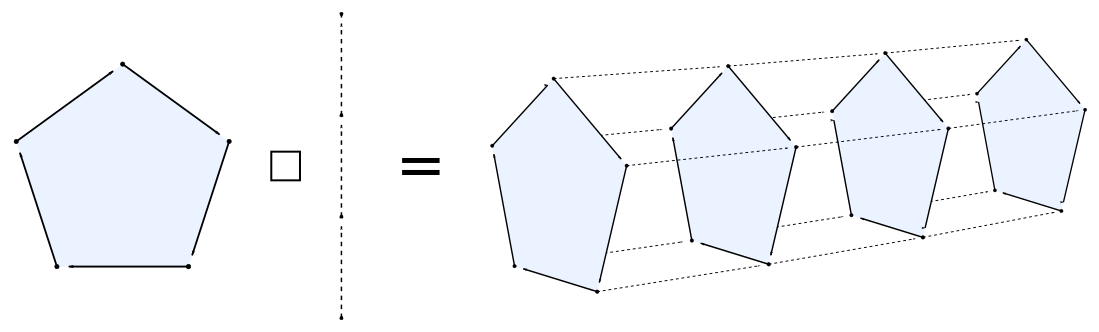
\includegraphics[scale=0.36]{fig/graph-product.pdf}}
\caption{The Cartesian graph product of \hs{pentagon} and \hs{p4}.\label{fig-product}}
\end{figure*}

As another application of \hs{gmap}, we implement the \emph{Cartesian graph
product} operation \hs{box}, or $G~~\square~~H$, where the resulting vertex set is
$V_G \times V_H$ and vertex $(x, y)$ is connected to vertex $(x', y')$ if
either $x = x'$ and $(y, y') \in E_H$, or $y = y'$ and $(x,x')\in E_G$. An example of the Cartesian product of graphs \hs{pentagon}
and \hs{p4} is shown in Fig.~\ref{fig-product}.

\begin{minted}{haskell}
box :: (Graph g, Vertex g @\teq@ (a, b))
    => GraphFunctor a -> GraphFunctor b -> g
box x y = @\std{foldr}@ overlay empty $ xs ++ ys
  where
    xs = @\std{map}@ (\b -> gmap (,b) x) . toList $ gmap id y
    ys = @\std{map}@ (\a -> gmap (a,) y) . toList $ gmap id x
\end{minted}

The Cartesian product $G~~\square~~H$ is assembled by creating $|V_H|$ copies
of graph $G$ and overlaying them with $|V_G|$ copies of graph $H$. We get
access to the list of graph vertices using \hs{toList} and turn vertices of
original graphs into pairs of vertices by \hs{gmap}. Note that we need to
\emph{reinterpret} the input of type \hs{GraphFunctor} as a polymorphic graph
by \hs{gmap@\,id@} before passing it to the \hs{toList} function, which expects
inputs of type \hs{ToList}. As you can see, we managed to implement quite
a sophisticated graph transformation function \hs{box} fully polymorphically.
One can go further up in layers of abstraction and use \hs{box} to construct
\emph{mesh} and \emph{torus} graphs as
\hs{mesh xs ys = box (path xs) (path ys)} and
\hs{torus xs ys = box (circuit xs) (circuit ys)}, respectively.

The \hs{toList} function is implemented as follows:

\begin{minted}{haskell}
newtype ToList a = L { toList :: [a] }
\end{minted}
\vspace{1mm}
\begin{minted}{haskell}
instance Graph (ToList a) where
     type Vertex (ToList a) = a
     empty       = L $ [@@]
     vertex  x   = L $ [x]
     overlay x y = L $ toList x ++ toList y
     connect x y = L $ toList x ++ toList y
\end{minted}

\noindent
Note that we do not provide the \hs{Eq} instance for \hs{ToList}, because it
is impossible to make it law-abiding without requiring \hs{Eq} for vertices,
and we would like to avoid this in order to keep the \hs{box} type signature
fully parametric. As a consequence, \hs{toList (1 + 1)} produces the
list \hs{[1,1]}.

\subsection{Graph monad}\label{sub-monad}

What do the operations of removing a vertex and splitting a vertex have in common?
They both can be implemented by replacing each vertex of a graph with a (possibly empty)
subgraph and flattening the result. You may recognise this as the \hs{bind} operation
of a monad. We implement \hs{bind} by wrapping it into yet another \hs{newtype}:

\begin{minted}{haskell}
newtype GraphMonad a =
    M { bind :: forall g. Graph g => (a -> g) -> g }
\end{minted}
\vspace{1mm}
\begin{minted}{haskell}
instance Graph (GraphMonad a) where
    type Vertex (GraphMonad a) = a
    empty       = M $ \_ -> empty
    vertex  x   = M $ \f -> f x
    overlay x y = M $ \f -> overlay@\,@(bind x f)@\,@(bind y f)
    connect x y = M $ \f -> connect@\,@(bind x f)@\,@(bind y f)
\end{minted}

The implementation is almost identical to \hs{gmap}: instead of
wrapping the value \hs{f@\,\,@x} into a \hs{vertex}, we should just leave it as is.
Let us see how we can make use of this new type in our toolbox.

Firstly, we are going to implement a \hs{@\std{filter}@}-like function \hs{induce}
that, given a vertex predicate and a graph, will compute the \emph{induced subgraph}
on the set of vertices that satisfy the predicate by turning all other
vertices into empty subgraphs and flattening the result.

\begin{minted}{haskell}
induce :: Graph g
    => (Vertex g -> Bool) -> GraphMonad (Vertex g) -> g
induce p g = bind g $
    \v -> if p v then vertex v else empty
\end{minted}
\vspace{1mm}
\begin{minted}[frame=single,fontsize=\small]{haskell}
@\ghci@ edgeList $ induce (<3) $ clique [0..10]
[(0,1),(0,2),(1,2)]
\end{minted}

\noindent
As you can see, by inducing a clique on a subset of the vertices
that we like \hs{(<3)}, we get a smaller clique, as expected.
The cost of \hs{induce} for a given expression $g$ is $O(|g|)$.

Now we can implement the \hs{removeVertex} function:

\begin{minted}{haskell}
removeVertex :: (Graph g, Eq (Vertex g))
    => Vertex g -> GraphMonad (Vertex g) -> g
removeVertex v = induce (/= v)
\end{minted}
\vspace{1mm}
\begin{minted}[frame=single,fontsize=\small]{haskell}
@\ghci@ edgeList $ removeVertex 2 $ 1 * 2 + 3 * 1
[(3,1)]
\end{minted}

The polymorphic implementation of \hs{removeVertex} presented above takes
$O(|g|)$ to remove a vertex from a graph expression $g$, which is
slower than some concrete graph data structures.

We can also use the \hs{bind} function to split a vertex into a list of given vertices:

\begin{minted}{haskell}
splitVertex :: (Graph@\,\,g@,@\,@Eq@\,@(Vertex@\,\,g@)) => Vertex@\,\,g@
    -> [Vertex@\,\,g@] -> GraphMonad@\,@(Vertex@\,\,g@) -> g
splitVertex v vs g = bind g $
    \u -> if u == v then vertices vs else vertex u
\end{minted}
\vspace{1mm}
\begin{minted}[frame=single,fontsize=\small]{haskell}
@\ghci@ edgeList $ splitVertex 1 [0, 1] $ 1 * (2 + 3)
[(0,2),(0,3),(1,2),(1,3)]
\end{minted}

\noindent
Here vertex 1 is split into a pair of vertices $\{0, 1\}$ that have the same connectivity.

\subsection{Beyond homomorphisms}\label{sub-beyond}

Most of the \hs{newtype} wrappers defined in this section are \emph{homomorphisms},
that is, they preserve the structure of the original graph expression. The two
exceptions are: \hs{Transpose}, which is an \emph{antihomomorphism}, and
\hs{ToList} which collapses the structure of the original expression into a list.

Below we derive an implementation for \hs{removeEdge}, which is another
example of a useful function that is not a homomorphism. Removing an edge sounds
easy, but the result is the most complicated \hs{newtype} in this paper.

\begin{figure*}
\begin{minted}{haskell}
            newtype RemoveEdge a = RE { re :: forall g. (Vertex g @\teq@ a, Graph g) => a -> a -> g }
\end{minted}
\vspace{1mm}
\begin{minted}{haskell}
            instance Eq a => Graph (RemoveEdge a) where
                type Vertex (RemoveEdge a) = a
                empty       = RE $ \_ _ -> empty
                vertex  x   = RE $ \_ _ -> vertex x
                overlay x y = RE $ \u v -> overlay (re x u v) (re y u v)
                connect x y = RE $ \u v -> connect (removeVertex u $ re x u u) (re y u v) `overlay`
                                           connect (re x u v) (removeVertex v $ re y v v)
\end{minted}
\vspace{0mm}
\begin{minted}{haskell}
            removeEdge :: (Eq (Vertex g), Graph g) => Vertex g -> Vertex g -> RemoveEdge (Vertex g) -> g
            removeEdge u v g = re g u v
\end{minted}
\caption{Removing an edge from a polymorphic graph.}
\end{figure*}

\noindent
Here is how it works. Removing an edge $(u,v)$ from the \hs{empty} graph
or a \hs{vertex} is easy:
nothing needs to be done, because there are no edges. To remove the edge from an
\hs{overlay}, we simply recurse to both subexpressions, because the overlay does not create
any edges. The \hs{connect} case $x \rightarrow y$ is handled by overlaying two graphs:
$x_u \rightarrow y_{uv}$ and $x_{uv} \rightarrow y_v$, where:

\begin{itemize}
    \item $x_u = \hs{removeVertex}~u~x$ and $y_{uv} = \hs{removeEdge}~u~v~y$,
    thus $x_u \rightarrow y_{uv}$ definitely does not contain the edge $(u,v)$
    at the cost of losing the vertex $u$ in the left-hand side $x_u$.
    \item $y_v = \hs{removeVertex}~v~y$ and $x_{uv} = \hs{removeEdge}~u~v~x$,
    thus $x_{uv} \rightarrow y_v$ definitely does not contain the edge $(u,v)$
    at the cost of losing the vertex $v$ in the right-hand side $y_v$.
\end{itemize}
\noindent
The overlay $x_u \rightarrow y_{uv} + x_{uv} \rightarrow y_v$ contains the
vertices $u$ and $v$, because at least one copy of each vertex has been preserved,
but the edge $(u,v)$ is removed in both subexpressions as intended.

We demonstrate \hs{removeEdge} on two simple examples:
\begin{minted}[frame=single,fontsize=\small]{haskell}
@\ghci@ edgeList $ path "Hello"
[('H','e'),('e','l'),('l','l'),('l','o')]

@\ghci@ edgeList $ removeEdge 'H' 'e' $ path "Hello"
[('e','l'),('l','l'),('l','o')]

@\ghci@ edgeList $ removeEdge 'l' 'l' $ path "Hello"
[('H','e'),('e','l'),('l','o')]
\end{minted}

\noindent
The \hs{removeEdge} function is expensive: given an expression of size $|g|$
it may produce a transformed expression of the quadratic size $O(|g|^2)$. Many
concrete \hs{Graph} instances provide much faster equivalents of \hs{removeEdge}.

\begin{figure*}
\centerline{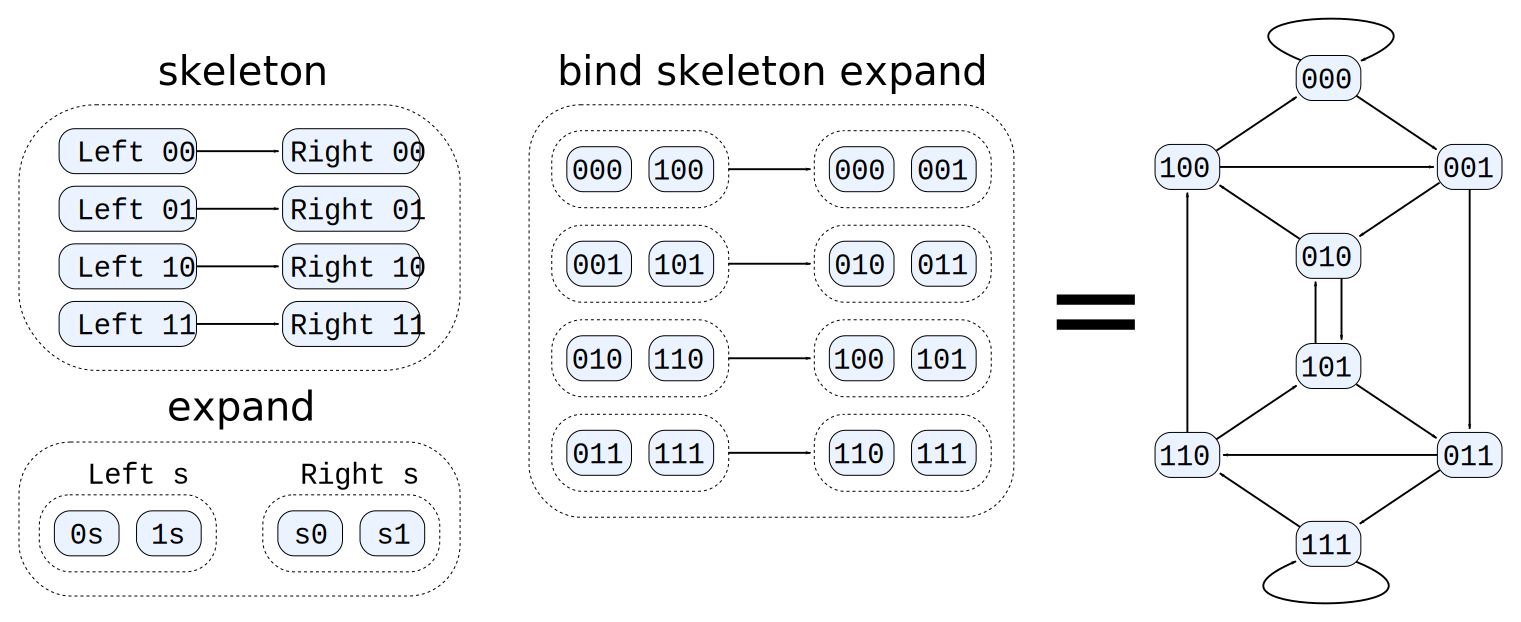
\includegraphics[scale=0.3]{fig/De-Bruijn-construction.pdf}}
\caption{Constructing De Bruijn graphs using the graph monad.\label{fig-de-bruijn}}
\end{figure*}

\subsection{De Bruijn graphs}

To demonstrate that one can easily construct sophisticated graphs using
the presented library, let us try it on \emph{De Bruijn graphs}, an interesting
combinatorial object that frequently shows up in computer engineering and
bioinformatics. The implementation is very short, but requires some explanation:

\begin{minted}{haskell}
deBruijn :: (Graph g,@\,@Vertex g @\teq@ [a])@\,@=>@\,@Int -> [a] -> g
deBruijn len alphabet = bind skeleton expand
  where
    overlaps = @\std{mapM}@ (@\std{const}@ alphabet) [2..len]
    skeleton = edges [@\,@(Left s,@\,@Right s) | s@\,@<-@\,\blk{overlaps}\,@]
    expand v = vertices
        [ @\std{either}@ ([a]++) (++[a]) v | a <- alphabet ]
\end{minted}

The function builds a De Bruijn graph of dimension \hs{len} from symbols of the given
\hs{alphabet}. The vertices of the graph are all possible words of length \hs{len}
containing symbols of the \hs{alphabet}, and two words are connected $x \rightarrow y$
whenever $x$ and $y$ match after we remove the first symbol of $x$ and the last symbol
of $y$ (equivalently, when $x = az$ and $y = zb$ for some symbols $a$ and $b$).
The process of construction of a 3-dimensional De Bruijn graph on the alphabet
$\{0, 1\}$ is illustrated in Fig.~\ref{fig-de-bruijn}. Here are all the ingredients
of the solution:
\begin{itemize}
    \item \hs{overlaps} contains all possible words of length \hs{len-1} that
    correspond to overlaps of connected vertices.
    \item \hs{skeleton} contains one edge per overlap, with \hs{Left} and
    \hs{Right} vertices acting as temporary placeholders.
    \item We replace a vertex \hs{Left@\,$s$@} with a subgraph of two vertices
    $\{0s, 1s\}$, i.e. the vertices whose suffix is $s$. Symmetrically,
    \hs{Right@\,$s$@} is replaced by vertices $\{s0, s1\}$. This is captured
    by the function \hs{expand}.
    \item The result is obtained by computing \hs{bind} \hs{skeleton} \hs{expand}.
\end{itemize}

Below we construct the De Bruijn graph shown in Fig.~\ref{fig-de-bruijn}.
\begin{minted}[frame=single,fontsize=\small]{haskell}
@\ghci@ edgeList $ deBruijn 3 "01"
[("000","000"),("000","001"),("001","010"),("001","011")
,("010","100"),("010","101"),("011","110"),("011","111")
,("100","000"),("100","001"),("101","010"),("101","011")
,("110","100"),("110","101"),("111","110"),("111","111")]

@\ghci@ g = deBruijn 9 "abc"
@\ghci@ all (\(x,y) -> drop 1 x == dropEnd 1 y) $ edgeList g
True

@\ghci@ Set.size $ domain g
19683 -- i.e. 3^9

@\ghci@ Set.size $ relation g
59049 -- i.e. 3^10
\end{minted}

\noindent
Note that a De Bruijn graph of dimension \hs{len} on the \hs{alphabet} has
$|\hs{alphabet}|^{\hs{len}}$ vertices and $|\hs{alphabet}|^{\hs{len} + 1}$
edges.

\subsection{Summary}\label{sub-library-summary}

We have presented a library of polymorphic graph construction and
transformation functions that provide a flexible and elegant way to manipulate
graph expressions polymorphically. Polymorphic graphs are highly reusable
and composable, and can be interpreted using any of the \hs{Graph} instances
defined in~\S\ref{sec-a-la-carte}, as well as other instances provided by the
\textsf{algebraic-graphs} library that is available on Hackage.
The library is written in the vanilla functional programming style and has
no dependencies apart from core GHC libraries.
Many of the presented graph transformation algorithms are expressed using familiar
functional programming abstractions, such as functors and monads.

%!TEX root = alga.tex
\section{Related work}\label{sec-related}

% In this section we review existing approaches to working with graphs developed
% by the functional programming community.

% \begin{itemize}
%     \item Tying the knot:
%     \item Borrowing imperative algorithms via the State monad.
%     \item Data.Graph by King & Launchbury, 1995. \url{https://galois.com/wp-content/uploads/2014/08/pub_JL_StructuringDFSAlgorithms.pdf}.
%     Clever tricks exploiting lazy evaluation (Johnsson 1998) \url{https://pdfs.semanticscholar.org/a6ed/4e55f148e0c48445269990102838f7d7abb5.pdf?_ga=1.176470501.1134931652.1487554701}

%     \item Inductive Graphs by Martin Erwig, 2001. \url{https://web.engr.oregonstate.edu/~erwig/papers/InductiveGraphs_JFP01.pdf}
%     \item Structured Graphs by Oliveira & Cook. \url{https://www.cs.utexas.edu/~wcook/Drafts/2012/graphs.pdf}
%     \item An initial-algebra approach to directed acyclic graphs, by J. Gibbons
%     \item "Algebras for graphs have been studied in the context of graph rewriting, see Bauderon and Courcelle (1986), for example."
% \end{itemize}

%!TEX root = alga.tex
\section{Discussion and future work}\label{sec-discussion}

% Using discrimination library for better efficiency
% Modular decomposition for minimisation
% Solving graph equations


%% Acknowledgments
\begin{acks}
  I would like to thank Arseniy Alekseyev and Neil Mitchell
  for numerous discussions on algebraic graphs, their advice,
  criticism and encouragement. Without their help this work would
  have likely remained an unfinished toy project.
  Simon Peyton Jones, Brent Yorgey, Danil Sokolov, Ben Lippmeier, Ulan Degenbaev
  and several anonymous reviewers provided constructive feedback on an
  earlier draft of this paper, helping to substantially improve it. Last but
  not least, I'm very grateful to Victor Khomenko for his contribution to the
  algebra of parameterised graphs that forms the mathematical foundation of this work.
\end{acks}

\bibliography{publications}

\end{document}
